%% LyX 2.3.4.2 created this file.  For more info, see http://www.lyx.org/.
%% Do not edit unless you really know what you are doing.
\documentclass[english]{article}
\usepackage[T1]{fontenc}
\usepackage[latin9]{inputenc}
\usepackage{verbatim}
\usepackage{float}
\usepackage{textcomp}
\usepackage{graphicx}

\makeatletter

%%%%%%%%%%%%%%%%%%%%%%%%%%%%%% LyX specific LaTeX commands.
%% A simple dot to overcome graphicx limitations
\newcommand{\lyxdot}{.}


%%%%%%%%%%%%%%%%%%%%%%%%%%%%%% User specified LaTeX commands.
\usepackage{multirow}
%\usepackage{table}
%\usepackage{tabular}

\makeatother

\usepackage{babel}
\begin{document}
\title{Prediction of Protein-Protein Interactions on the Human and Rice Interactomes}
\author{Nicol�s L�pez-Rozo\thanks{Pontificia Universidad Javeriana Cali, ORCID: 0000-0002-8060-6891\protect \\
\protect\hphantom{ema.}email: nicolaslopez@javerianacali.edu.co}, Jorge Finke\thanks{Pontificia Universidad Javeriana Cali, ORCID: 0000-0003-2393-6066},
Camilo Rocha\thanks{Pontificia Universidad Javeriana Cali, ORCID: 0000-0003-4356-7704}}
\maketitle
\begin{abstract}

A recent study in network-based prediction of protein-protein interactions
(PPIs) reveals that two proteins are more likely to interact, the
higher the number of paths of length 3 between them (normalized by
the geometric average of their interactions). This paper extends previous
work on mapping binary interactions by taking into account the learning
of features (embeddings) of the PPI network. In particular, we implement
a gradient boosted decision tree model (\texttt{XGBoost}) using handcrafted
features (including the normalized measure) and embeddings from an
algorithm that generates a low-dimensional representation of nodes
(\texttt{Node2Vec}). Our main result shows that while the measure
remains an important feature for predicting interactions, better performance
is achieved when in addition embedding features are considered. The
proposed approach is validated for the human and rice interactomes.
For both cases, the combination of both types of features yield higher
AUC values. The developed framework can also be applied to interactomes
of other organisms for which PPI networks have recently become available.
\end{abstract}

\section{Introduction}

Proteins are key actors of biological processes inside cells. Rather
than carrying out tasks as single agents, they are part of dynamic
networks of protein-protein interactions (PPI) \cite{Lin2017}. Such
networks underlie a variety of interdependent mechanisms, including
signal transduction, homeostasis control and stress responses. Furthermore,
PPI networks play an important role in physiological and developmental
processes such as protein phosphorylation, transcriptional co-factor
recruitment and transporter activation \cite{Zhang_2010_PPI}.

A common way to create PPI networks (or validate particular protein-protein
interactions) is the \emph{Yeast-Two-Hybrid} technique (also known
as \emph{two-hybrid screening} or \emph{Y2H}). Figure \ref{Y2H}A
illustrates the biological basis of Y2H: the expression of a specific
reporter gene is activated by the binding of a DNA-binding Domain
(DB) and an Activation Domain (AD) of a Transcription Factor, which
in turn binds to an Upstream Activation Sequence (UAS). To evaluate
an interaction between two proteins, the Y2H approach fuses one protein
to the DB domain (known as \emph{bait}) and another protein to the
AD (known as \emph{prey}). If the proteins interact, the reporter
gene expression is activated by the AD (Fig. \ref{Y2H}B). Otherwise,
if proteins fail to interact, the reporter gene is not expressed (Fig.
\ref{Y2H}C).

\begin{figure}[h]
\caption{\label{Y2H}The Yeast-2-Hybrid technique offers an experimental approach
for constructing PPI networks.}

\noindent \centering{}\includegraphics[width=0.7\columnwidth]{Y2H}
\end{figure}

Based on the outcome of numerous Y2H experiments, undirected networks
of interactions between proteins can be constructed. However, relying
only on experimental validation of PPIs is detrimental to research
due to its hindrance in costs, accuracy, required manpower and time
\cite{Laraia2015PPI,Macalino2018PPI}. Besides, the number of missing
interactions for pairs of proteins on many organisms leverage the
usage of computational methods for prediction of such interactions.
\begin{comment}
The focus of this study is to evaluate different methods for predicting
PPIs using the network of known interactions. 
\end{comment}

A common way of predicting interactions is usually based on social
networks analysis, more specifically on the triadic closure principle
(TCP). TCP states that the higher the number of common neighboring
nodes between two nodes, the higher the probability that they interact
\cite{Goldberg2003SmallWorld}. TCP can be addressed mathematically
by counting the number of shared neighbors of a pair of nodes, also
known as the Common Neighbors algorithm. By raising the adjacency
matrix (A) of the network to the second power (A\texttwosuperior ),
TCP can be considered for further analyses. However, previous studies
show that the mentioned approach usually fails because it does not
consider the structural and chemical properties of the proteins \cite{Cannistraci2013Networks,Kovacs2019}.

A variety of methods for predicting interactions in PPI networks have
been proposed in recent years \cite{Chang2016PPI,Chen2019PPI,Kotlyar2015PPI}.
Kovacs et al (2019) introduce a network-based approach which predicts
the interaction between two proteins based on the number of paths
of length 3, normalized by the geometric average of their interactions.
The simplest mathematical representation of this principle consists
on the third power of the adjacency matrix (A\textthreesuperior ).
Furthermore, Kovacs et al present a degree-normalized scaling for
this metric, which reduces bias caused by intermediate hubs within
the paths of length 3. This handcrafted measure, denoted L3, enables
the proposed approach to outperform previous methods for predicting
binary protein interactions in yeast (\emph{S. cerevisiae}), Arabidopsis
(\emph{A. thaliana}), worm (\emph{C. elegans}), fly (\emph{D. melanogaster}),
fission yeast (\emph{S. pombe}), mouse (\emph{M. musculus}) and humans
\cite{Kovacs2019}.

\begin{comment}
JF: Yet you do more than evaluating this three measures so this has
to be updated.

NL: Done!

JF: Not sure we should use L3 above since it is being redefined as
a normalized measure here!

JF{*}: state what the results are: ``The contributions of this paper
are...''

Which article predicts PPI based on TCP? add refs
\end{comment}

The focus of this study is to evaluate different methods for predicting
PPIs using the network of known interactions. To achieve this, human
and rice PPI networks are compared using the proposed methods (A2,
A3, L3), as well as a low-dimensional representation of nodes (\texttt{Node2Vec})\cite{Grover_2016}.
After that, combinations of the two types of methods are tested. In
the case of the human network, two different versions of the human
interactome \cite{Rolland2014Human} are used for training and another
interactome version is used for validation (\emph{HI-III})\cite{Kovacs2019}.
For the rice interactome, a portion of the known interactions removed
and then predicted with different techniques based on the known interactions.
The main contributions of this paper are i) a general framework for
link prediction in non-directed networks and ii) two applications
of this framework to biological networks with a structural insight.

The remainder of this paper is organized as follows. Section 2 describes
the methodological steps and key milestones in the preparation of
the networks, model parameters and experimental configurations. Section
3 presents the main results of the models for the human and rice interactomes.
Section 4 presents the main conclusions of this study. Finally, Appendix
presents supplementary information and figures which complement the
results described in this paper.

\section{Materials and Methods}

\subsection{Data Availability}

The human interactome data was downloaded from the repository of the
length-3 degree normalized paths methodology \cite{Kovacs2019}: the
dataset \emph{HI-II-14} and \emph{HI-TESTED} are used for prediction.
The dataset \emph{HI-III} is available in the same repository and
is used for validation.

The rice interactome information was downloaded from the STRING database
\cite{Szklarczyk2019}, corresponding to the subspecies \emph{Oryza
sativa}. The file contains more than 8 million PPIs from several sources.
For the purpose of this study, only PPIs with evidence from curated
databases are used. The resulting network contains $5025$ nodes and
$164420$ edges.

\subsection{Code Implementation}

The original code implementation in \texttt{C++} from Kovacs et al
(2019) was adapted to \texttt{Python} (V3.6). For the purpose of algorithmic
validation, the three methods were implemented from scratch with basic
functionalities and data structures of the \texttt{Python} language.
The code is publicly available under the repository github.com/ocinlr/PPIPL3.

\subsection{Data Preprocessing}

Information for the human interactome was used as-is, which corresponds
to networks of $4298$, $3727$ and $5604$ proteins and $13868$,
$9433$ and $23322$ interactions, respectively.

For the rice interactome, an additional preprocessing was performed.
The filtered network for rice consists of $5025$ proteins (nodes)
and $164420$ interactions (edges) distributed among $178$ connected
components. The connected component with the greatest number of edges
was selected. The extracted connected component consists of $n=4390$
nodes and $m=163319$ edges, which corresponds to $99.33$\% of edges.

\subsection{Edge Prediction}

For predicting interactions for each network, the algorithms described
below were used. It is important to keep in mind how the PPI network
$G=(V,E)$ is conceptualized: each node ($v_{i}\in V$) represents
a protein and each undirected edge ($e_{b}=\{v_{i},v_{j}\},\,e_{b}\in E$)
represents an interaction among proteins $v_{i}$ and $v_{j}$.
\begin{description}
\item [{Common~Neighbors~(A2)}] This method is based on the Triadic Closure
Principle which states that the more common friends two individuals
have, the more likely that they know each other. For implementing
this measure, $A{{}^2}$ matrix is calculated, where $A$ is the adjacency
matrix of the network.
\item [{Length-3~Path~Counts~(A3)}] This is a simple implementation
of the notion of ``if my friends and your friends interact, then
we might interact too''. For implementing this measure, $A{{}^3}$
is calculated.
\item [{Degree-normalized~L-3~Score~(L3)}] The previous approach might
overestimate the importance of some edges due to intermediate hubs
which add many shortcuts in the graph. To address that issue, a degree
normalization for the path $v_{i}\rightarrow v_{m}\rightarrow v_{n}\rightarrow v_{j}$
is applied by considering the degree of the intermediate nodes $k_{m}$
and $k_{n}$, as follows.
\[
p_{i,j}=\sum_{m,n\in|V|}\frac{A_{i,m}\cdot A_{m,n}\cdot A_{n,j}}{\sqrt{k_{m}\cdot k_{n}}}
\]
\\
where $A_{i,j}$ represents the value of the adjacency matrix for
nodes $i$ and $j$.
\end{description}

\subsection{Sampling Procedure}

For each PPI network, the following procedure was performed 10 times
to address the stochastic nature of the process:
\begin{enumerate}
\item A percentage of interactions is removed at random from the network
(20\%).
\item The same amount of removed interactions are then predicted using the
main methods for prediction mentioned by Kovacs et al (2019): Common
Neighbors (\textbf{A2}), raw path count of paths of length 3 (\textbf{A3})
and the Length-3 degree-normalized score (\textbf{L3}).
\item A test dataset is created as follows: all removed edges are included
(as observed positives for the ML algorithm) and from the predicted
edges of \textbf{A2}, \textbf{A3} and \textbf{L3} that don't lie in
the previous classification (observed negatives), a random subset
is chosen such that the dataset is balanced, that is, the amount of
observed positive labels is equal to the observed negative labels.
\item Once the dataset is ready, it is randomly partitioned: 80\% is used
for \texttt{XGBoost} model training and 20\% is used for validation.
It is important to have in mind that balanced distribution of the
positive and negative labels in the datasets was satisfied in training,
but validation is performed using the remaining unbalanced data.
\end{enumerate}
It is worth mentioning that some exploration experiments were carried
out with interactions removal percentages of 2, 5, 10 and 20\%, as
well as train-test partitions of 15-85, 80-20 and 75-25, and the explained
parameter set was selected because it either represented a marginal
gain (results not shown) or because it was a common parameter selection
in related literature.

\subsection{Feature Extraction with \texttt{Node2Vec}}

The \texttt{Node2Vec} module was used for extracting features of the
interactomes. The considerations for the model were:
\begin{itemize}
\item All paths in the random walks are equally likely.
\item Use a modest number of dimensions and threads for calculation.
\item Since length-3 paths are the defining property in this study, there
is no necessity for longer walks. However, it is important to try
out many possible redundant routes and to consider a window of at
least 4.
\item Other standard parameters were left with default values.
\item Edge embeddings were calculated using a geometric ratio of the node
embeddings.
\end{itemize}

\subsection{Handcrafted Features}

Due to the poor results of the \emph{raw} Length-3 counting (\textbf{A3}),
a different approach for this information was carried out: As it still
gives a lot of information that might be useful for a predictive routine,
this counting was normalized (dividing by the greatest counting in
the \textbf{A3} top predictions) and then used as a feature for the
Machine Learning algorithm. For completeness, \textbf{A2} and \textbf{L3}
measures were used as a input features. Finally, the case were no
handcrafted feature was also considered, that is, only the features
extracted from the structure of the network were considered.

\subsection{Feature to Predict: Existence}

The feature to predict corresponds to the possible existence (\emph{True/False})
of a link based on the existing information of the network. This is
evaluated by taking out a fraction of the edges and then trying to
predict for a given set of possible edges if they have a high probability
to belong to the original network.

\subsection{Machine Learning Algorithm}

The Extreme Gradient Boosting implementation of gradient boosted trees
is applied to evaluate the existence of an edge. Gradient boosted
trees are usually used for supervised learning problems, where the
training data $X_{i}$ has multiple features and pretends to explain
(or predict) a target variable $Y_{i}$. The corresponding implementation
applied for this study is \texttt{XGBoost}.

\subsection{Result Validation}

As mentioned before, 80\% of the final dataset was randomly selected
and used for training, while the remaining information was used for
validation. The whole training-validation procedure was applied 10
times.

The chosen metric for validation was the Area under the Curve (\textbf{AUC})
of the Receiver Operating Characteristic (\textbf{ROC}). This curve
corresponds to plot the sensitivity (probability of predicting a real
positive as positive) against 1-specificity (probability of predicting
a real negative as positive). AUC values of 1 represent a perfect
prediction and 0.5 corresponds to a random guess. Normally, values
over 0.8 of AUC are considered good.

\section{Results and Discussion}

\subsection{Human Interactome}

As the first step in the evaluation of A2, A3 and L3 methods for link
prediction, the full calculation and ranking of all predictions was
carried out. The results for the analyzed human interactomes (\emph{HI-II-14}
and \emph{HI-TESTED}) is shown in Figure \ref{fig:HI1}, in which
the x axis represents a rank position $k$ and the y axis displays
the precision for the top $k$ predictions of each method, when assuming
interactome \emph{HI-III} as the validation set. 

\begin{figure}[h]
\caption{\label{fig:HI1}Methods Comparison for \emph{HI-II-14} and \emph{HI-TESTED}}

\noindent \centering{}\includegraphics[width=0.48\columnwidth]{hi-ii-14\lyxdot txt}\includegraphics[width=0.48\columnwidth]{hi-tested\lyxdot txt}
\end{figure}

As it can be inferred from the plots, L3-based predictions outperform
their $A{{}^2}$ counterparts. Results also show that L3-score and
$A^{3}$predictions follow a very similar trend.

However, it is of our interest to assess if Machine Learning can boost
the overall performance on the prediction, so the proposed procedure
was adapted to the human interactome data: Instead of having to remove
a fraction of edges from the network in order to predict and validate,
the prediction network and the validation networks are given beforehand.
The rest of the procedure is carried out as mentioned in Section 2.
Table \ref{T1} presents the results for the combinations of Node2Vec
with each feature.

\begin{table}
\caption{\label{T1}Summary statistics for human interactomes}
\includegraphics[width=1\columnwidth]{T1}
\end{table}

In general, performance of all models is above 0.96 in terms of F1-Score.
Although marginally, the A2 feature-enriched model for HI-TESTED performs
better than their counterparts based on paths of length 3. The opposite
is also true for HI-II-14: models enriched with L3 and A3 features
perform better than their A2 counterpart. Results for the Interactome
\emph{HI-II-14} with Node2Vec and each metric are presented in Figures
S\ref{HI1}, S\ref{HI2} and S\ref{HI3}. It can be seen that for
\emph{HI-II-14}, A2 performs marginally better than L3 when comparing
precision but worse in terms of recall, although all metrics have
AUC values of 0.99.

On the other hand, the interactome \emph{HI-TESTED} was assessed with
the same methodology as \emph{HI-II-14} and results are shown in Figures
S\ref{HI1-1}, S\ref{HI2-1} and S\ref{HI3-1}. For this interactome,
A2 performs better in terms of false positives than A3 and L3, but
in terms of false negatives, A3 actually performs better that A2 and
L3. In terms of AUC, metrics results are indistinguishable. 

An interesting assessment from this human datasets can be observed
when looking at the importance plots, which show a very biased influence
of the handcrafted features. Figure \ref{F8-importance-H1} shows
this behavior for the \emph{HI-II-14} dataset, which is very similar
to \emph{HI-TESTED} (Figure S\ref{F8-importance-H2}).

\begin{figure}[H]
\noindent \begin{centering}
\caption{\label{F8-importance-H1}Importance gain plots for \emph{HI-II-14}}
\par\end{centering}
\begin{centering}
\includegraphics[width=0.48\columnwidth]{Human/Imp\lyxdot A2\lyxdot 1}\includegraphics[width=0.48\columnwidth]{Human/Imp\lyxdot A3\lyxdot 1}
\par\end{centering}
\centering{}\includegraphics[width=0.48\columnwidth]{Human/Imp\lyxdot L3\lyxdot 1}
\end{figure}


\subsection{Rice Interactome}

For the rice interactome, different combinations of features were
trained on the model and validated. The results are shown in Table
\ref{T2}. First, prediction based on \texttt{Node2Vec} without any
additional feature included is used as baseline of comparison. Figure
\ref{F1} shows those results, and one can see that its mean performance
using the AUC is $0.93$. The results for all 10 repetitions of each
model are consistent, meaning the variance among each line is not
significant. The results for each model using only the default features
are satisfactory. This result can also be assessed when looking at
the confusion matrix, where a precision of $0.98$ and a recall of
$0.86$ are obtained.

\begin{table}
\caption{\label{T2}Summary statistics for rice interactome}
\includegraphics[width=1\columnwidth]{T2}
\end{table}

\begin{figure}[H]
\noindent \begin{centering}
\caption{\label{F1}Summary ROC curves for \texttt{Node2Vec} model alone}
\par\end{centering}
\noindent \raggedleft{}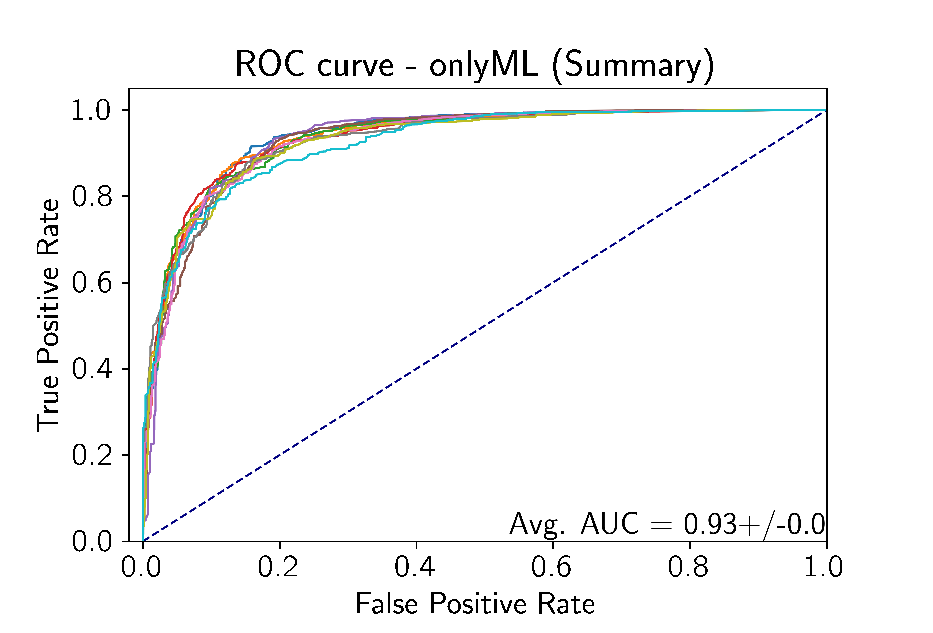
\includegraphics[width=0.48\columnwidth]{Only_ML/ROConlyML_SUMMARY}\includegraphics[width=0.48\columnwidth]{Only_ML/CMonlyML_SUMMARY}
\end{figure}

The next experiment carried out was to add for each prediction method
score as a prediction feature, that is, use the score as an additional
feature for the ML algorithm. Results for the Common Neighbors method
(\textbf{A2}), which uses paths of length 2, are shown in Figure S\ref{F2}.
All 10 experiments have small variability among them and perform better
than the baseline, with AUC of $0.98$. When looking at the confusion
matrix for this model, most guesses are true positives and true negatives,
resulting in a precision of $0.99$ and a recall of $0.91$. The same
analyses are done with the count of paths of length 3 (\textbf{A3})
and with the degree-normalized length-3 score (\textbf{L3}). These
results are presented in figures S\ref{F3} and \ref{F4}, respectively.
The corresponding AUC are $0.97$ and $0.98$.

\begin{figure}[H]
\noindent \begin{centering}
\caption{\label{F4}Results for \texttt{Node2Vec} with L3 feature}
\par\end{centering}
\noindent \raggedleft{}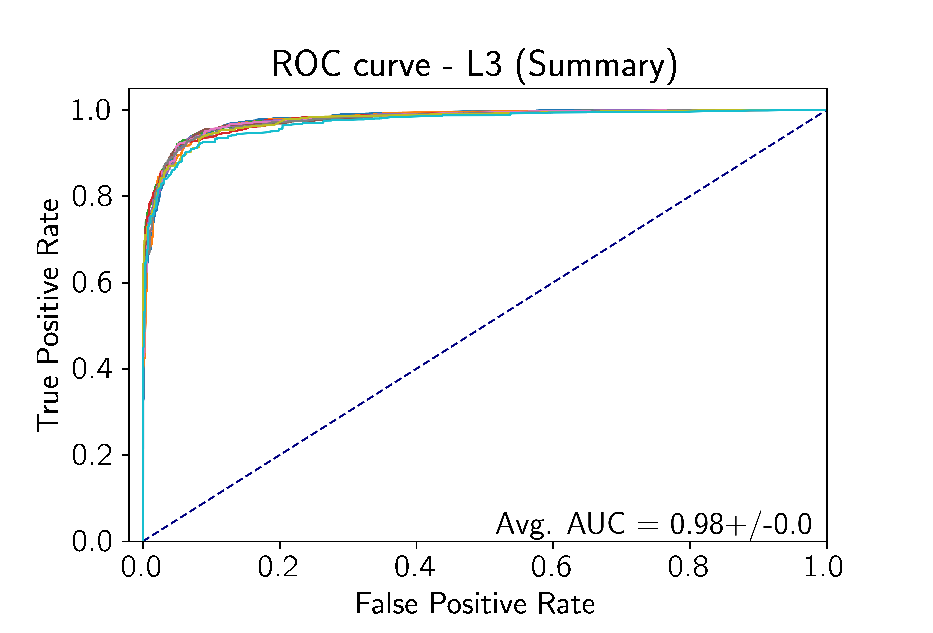
\includegraphics[width=0.48\columnwidth]{ML_Metric/ROCL3_SUMMARY}\includegraphics[width=0.48\columnwidth]{ML_Metric/CML3_SUMMARY}
\end{figure}

The precision when using the count of paths of length 3 (A3) is $0.99$
while the recall is $0.90$. It is interesting to observe that precision
decreased $0.16\%$ and recall decreased $0.58\%$. A similar situation
is obtained for the model with the normalized score (L3), whose precision
decreased to $0.99$ ($-0.08\%$) and recall decreased to $0.88$
($-2.38\%$). It can be seen also that the ROC curve achieves high
values of true positive rate sooner in the A2-featured model than
on the other models.

Another relevant assessment was carried out to verify the predictive
power of the metrics. \texttt{XGBoost} models were trained only using
each metric, for the same 10 experiments. Results are shown in Figures
S\ref{F5}, S\ref{F6} and \ref{F7}. XGBoost yields lower AUC values
when only considering A2, A3 and L3. Precision and recall for this
assessments, although lower than the previous experiments, are still
considered satisfactory.

\begin{figure}[H]
\noindent \begin{centering}
\caption{\label{F7}Results for L3 feature alone}
\par\end{centering}
\noindent \raggedleft{}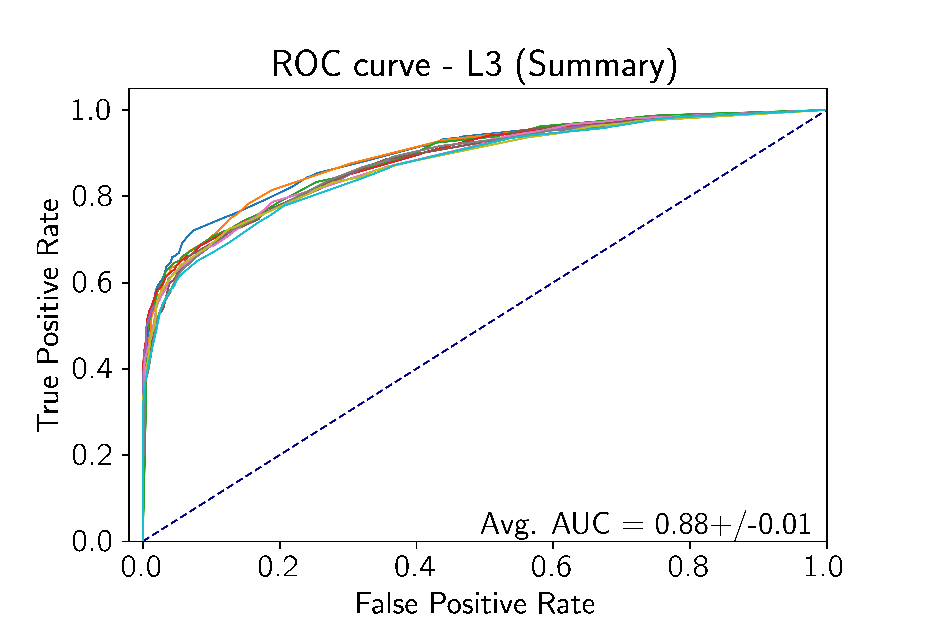
\includegraphics[width=0.48\columnwidth]{Only_Metric/ROConlyL3_SUMMARY}\includegraphics[width=0.48\columnwidth]{Only_Metric/CMonlyL3_SUMMARY}
\end{figure}

Finally, an relevant evaluation on the models that include a handcrafted
feature is necessary: How important is the appended feature for the
model result? The answer can be observed by the feature importance
plots for A2, A3 and L3 in Figure \ref{F8-importance}. Each plot
resembles the importance gain from each feature in the underlying
decision trees that \texttt{XGBoost} uses. Usually, the more bifurcations,
the higher gain a feature has, the more relevance a feature has on
the model prediction itself. All models have the appended feature
as the most important by a good margin, although margin for A3 is
not wide as for A2 or L3.

\begin{figure}[H]
\noindent \begin{centering}
\caption{\label{F8-importance}Importance gain plots for \texttt{Node2Vec}
with each feature}
\par\end{centering}
\begin{centering}
\includegraphics[width=0.48\columnwidth]{ML_Metric/Imp\lyxdot A2\lyxdot All}\includegraphics[width=0.48\columnwidth]{ML_Metric/Imp\lyxdot A3\lyxdot All}
\par\end{centering}
\centering{}\includegraphics[width=0.48\columnwidth]{ML_Metric/Imp\lyxdot L3\lyxdot All}
\end{figure}


\section{Conclusions}

Based on previous work from other authors\cite{Kovacs2019}, the intrinsic
knowledge of existing protein-protein interaction networks let scientists
elucidate promising new interactions to explore. In this study, a
machine learning algorithm was fed with previously elucidated information
about the network, as well as results form a state-of-the-art edge
embedding technique. Even if the baseline of the handcrafted features
(A2, A3, L3) yields good results, boosting that information with the
vector embedding, which calculates vector representations of the network
structure improves the overall performance of each method on its own.

On both human interactomes (\emph{HI-II-14} and \emph{HI-TESTED}),
applying \texttt{XGBoost} with the metrics yield results with high
AUC for the link prediction problem, and therefore this study extends
previous work by other authors that only consider the predictive power
of the metrics alone. In this case, the importance of the handcrafted
features was very significant and stands out of the Node2Vec features.

On the rice interactome, PPI prediction obtained high AUC values when
only using the node embedding technique (AUC=0.93) and when only using
the handcrafted features based on protein neighborhood (AUC \textasciitilde 0.88).
Even higher AUC results were achieved when the handcrafted features
and the vector representation information were combined (AUC \textasciitilde 0.98).

Importance values for the A3 method stand out less from the node embedding
information than in A2 and L3. However, handcrafted features are more
important for the prediction of the human than in the rice interactome. 

With this study, a framework for link prediction on protein-protein
interactions is presented and validated against the available information
on rice and human interactomes. However, it might be easily extended
to other organisms or even to other graphs not necessarily related
to biology, because the only required information is the network connectivity.
Satisfactory results might be expected when the framework is applied
to networks with a dense adjacency matrix, since calculations of L3
and Node2Vec rely on network exploration for an arbitrary node and
its degree.

\bibliographystyle{plain}
\bibliography{refs}

\pagebreak{}

\appendix

\part{Appendix}

\section{Supplementary Information}

\subsection{Datasets}

In the case of the human interactomes, the files were downloaded as-is
from the repository from Kovacs et al (2019). For the rice interactome,
the downloaded file was \emph{4530.protein.links.detailed.v11.0.txt.}
From this file, only interactions which have a curated origin (meaning
a value different than zero on the column \emph{'databases'}).

\subsection{Node2Vec Parameters}

For all experiments, the following parameters hold:
\begin{itemize}
\item For the (\texttt{p=1}, \texttt{q=1})
\item (\texttt{dimensions=16, workers=4})
\item (\texttt{walk\_length=5}, \texttt{num\_walks=300}, \texttt{window=5})
\item (\texttt{min\_count=1}, \texttt{batch\_words=4})
\item (\texttt{EdgeEmbedding=EdgeHadamardEmbedder})
\end{itemize}

\subsection{XGBoost parameters}
\begin{itemize}
\item \texttt{max\_depth=3}
\item \texttt{colsample\_bytree=0.6}
\item \texttt{eval\_metric=''auc''}
\end{itemize}

\section{Supplementary Figures}

\subsection{Human Interactome}

\begin{figure}[H]
\noindent \begin{centering}
\caption{\label{HI1}\emph{HI-II-14} results for \texttt{Node2Vec} with A2
feature}
\par\end{centering}
\noindent \raggedleft{}\includegraphics[width=0.48\columnwidth]{Human/ROC\lyxdot A2}\includegraphics[width=0.48\columnwidth]{Human/CM\lyxdot A2}
\end{figure}

\begin{figure}[H]
\noindent \begin{centering}
\caption{\label{HI2}\emph{HI-II-14} results for \texttt{Node2Vec} with A3
feature}
\par\end{centering}
\noindent \raggedleft{}\includegraphics[width=0.48\columnwidth]{Human/ROC\lyxdot A3}\includegraphics[width=0.48\columnwidth]{Human/CM\lyxdot A3}
\end{figure}

\begin{figure}[H]
\noindent \begin{centering}
\caption{\label{HI3}\emph{HI-II-14} results for \texttt{Node2Vec} with L3
feature}
\par\end{centering}
\noindent \raggedleft{}\includegraphics[width=0.48\columnwidth]{Human/ROC\lyxdot L3}\includegraphics[width=0.48\columnwidth]{Human/CM\lyxdot L3}
\end{figure}

\begin{figure}[H]
\noindent \begin{centering}
\caption{\label{HI1-1}\emph{HI-TESTED} results for \texttt{Node2Vec} with
A2 feature}
\par\end{centering}
\noindent \raggedleft{}\includegraphics[width=0.48\columnwidth]{Human/ROC\lyxdot A2\lyxdot 2}\includegraphics[width=0.48\columnwidth]{Human/CM\lyxdot A2\lyxdot 2}
\end{figure}

\begin{figure}[H]
\noindent \begin{centering}
\caption{\label{HI2-1}\emph{HI-TESTED} results for \texttt{Node2Vec} with
A3 feature}
\par\end{centering}
\noindent \raggedleft{}\includegraphics[width=0.48\columnwidth]{Human/ROC\lyxdot A3\lyxdot 2}\includegraphics[width=0.48\columnwidth]{Human/CM\lyxdot A3\lyxdot 2}
\end{figure}

\begin{figure}[H]
\noindent \begin{centering}
\caption{\label{HI3-1}\emph{HI-TESTED} results for \texttt{Node2Vec} with
L3 feature}
\par\end{centering}
\noindent \raggedleft{}\includegraphics[width=0.48\columnwidth]{Human/ROC\lyxdot L3\lyxdot 2}\includegraphics[width=0.48\columnwidth]{Human/CM\lyxdot L3\lyxdot 2}
\end{figure}

\begin{figure}[H]
\noindent \begin{centering}
\caption{\label{F8-importance-H2}Importance gain plots for \emph{HI-TESTED}}
\par\end{centering}
\begin{centering}
\includegraphics[width=0.7\columnwidth]{Human/Imp\lyxdot A2\lyxdot 2}
\par\end{centering}
\begin{centering}
\includegraphics[width=0.7\columnwidth]{Human/Imp\lyxdot A3\lyxdot 2}
\par\end{centering}
\centering{}\includegraphics[width=0.7\columnwidth]{Human/Imp\lyxdot L3\lyxdot 2}
\end{figure}


\subsection{Rice Interactome}

\begin{figure}[H]
\noindent \begin{centering}
\caption{\label{F2}Results for \texttt{Node2Vec} with A2 feature}
\par\end{centering}
\noindent \raggedleft{}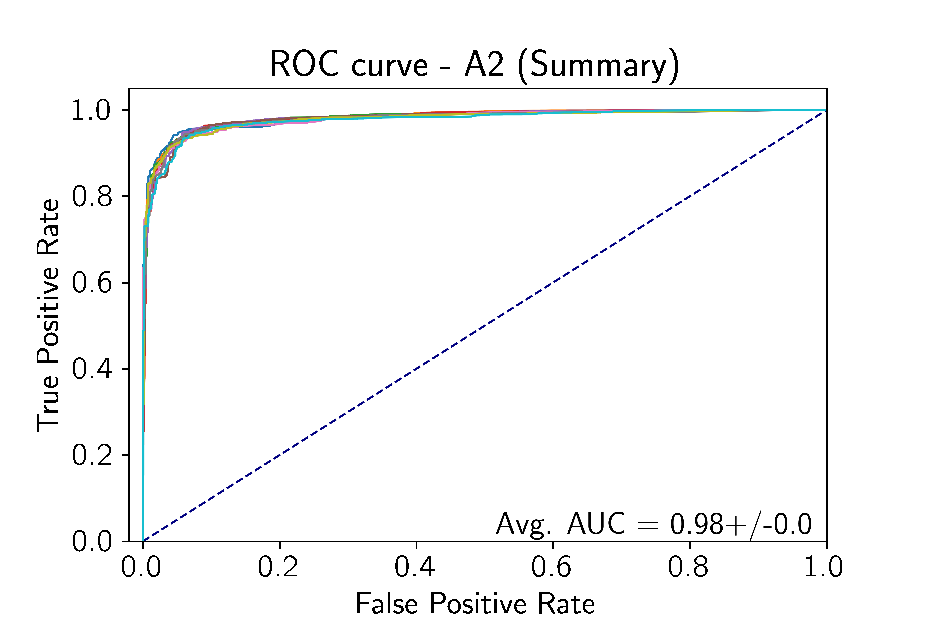
\includegraphics[width=0.48\columnwidth]{ML_Metric/ROCA2_SUMMARY}\includegraphics[width=0.48\columnwidth]{ML_Metric/CMA2_SUMMARY}
\end{figure}

\begin{figure}[H]
\noindent \begin{centering}
\caption{\label{F3}Results for \texttt{Node2Vec} with A3 feature}
\par\end{centering}
\noindent \raggedleft{}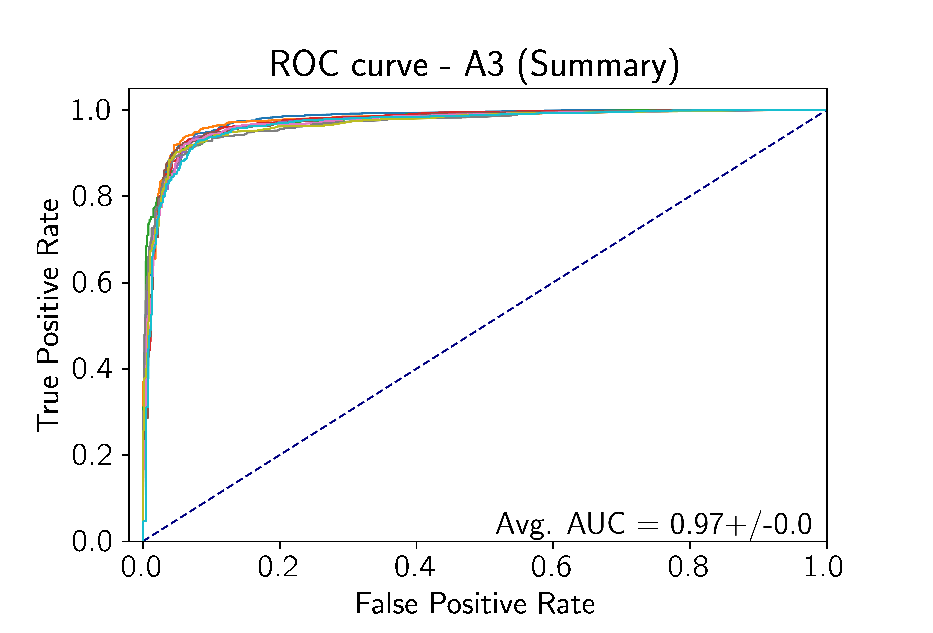
\includegraphics[width=0.48\columnwidth]{ML_Metric/ROCA3_SUMMARY}\includegraphics[width=0.48\columnwidth]{ML_Metric/CMA3_SUMMARY}
\end{figure}

\begin{figure}[H]
\noindent \begin{centering}
\caption{\label{F5}Results for A2 feature only}
\par\end{centering}
\noindent \raggedleft{}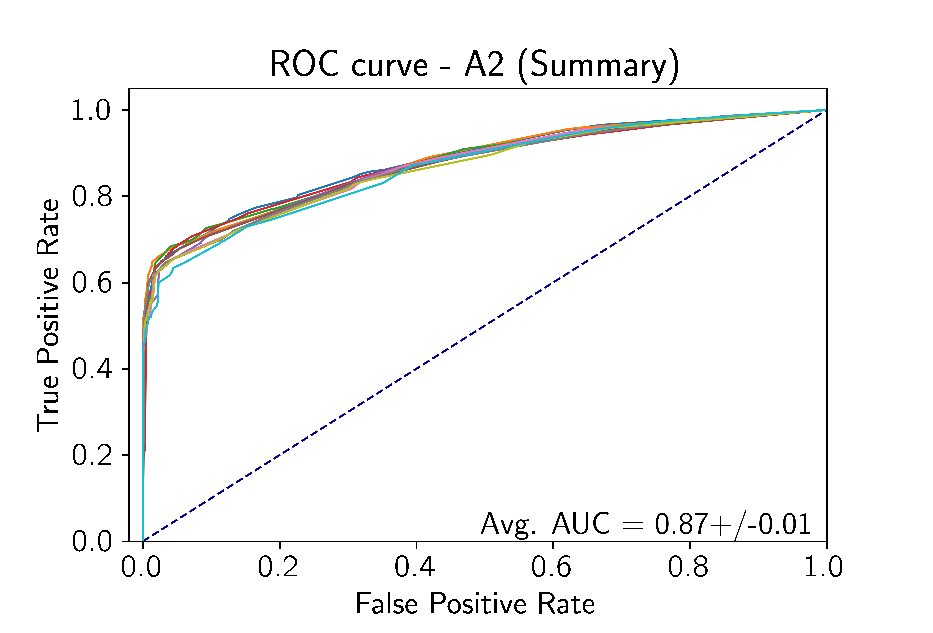
\includegraphics[width=0.48\columnwidth]{Only_Metric/ROConlyA2_SUMMARY}\includegraphics[width=0.48\columnwidth]{Only_Metric/CMonlyA2_SUMMARY}
\end{figure}

\begin{figure}[H]
\noindent \begin{centering}
\caption{\label{F6}Results for A3 feature alone}
\par\end{centering}
\noindent \raggedleft{}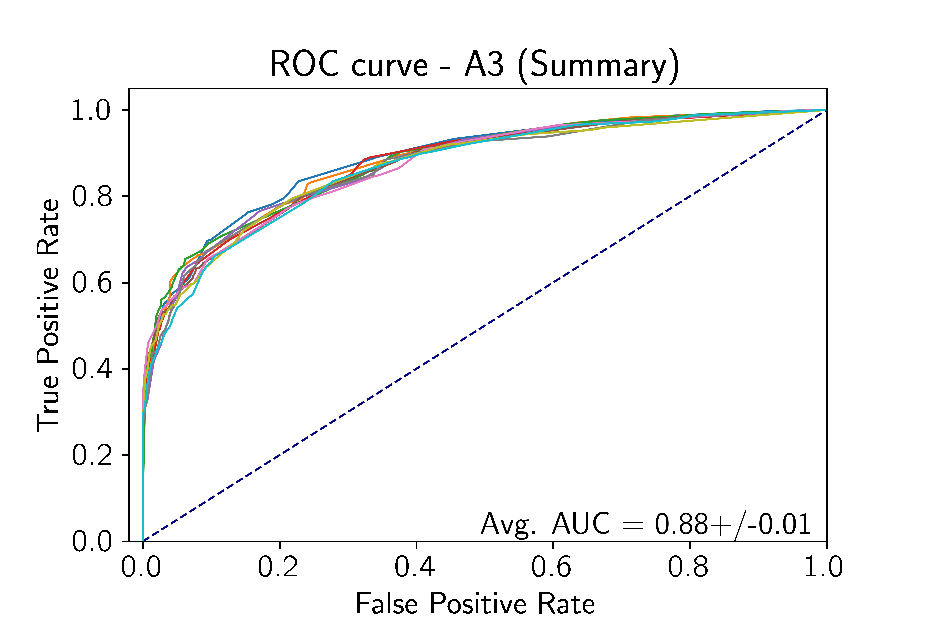
\includegraphics[width=0.48\columnwidth]{Only_Metric/ROConlyA3_SUMMARY}\includegraphics[width=0.48\columnwidth]{Only_Metric/CMonlyA3_SUMMARY}
\end{figure}

\end{document}
